\documentclass[aspectratio=169,xcolor=dvipsnames]{beamer}
\usetheme{Madrid}
\usecolortheme{seahorse}

\usepackage{graphicx}
\usepackage{amsmath}
\usepackage{booktabs}
\usepackage{tikz}
\usepackage{multirow}

% 自定义颜色
\definecolor{neuripsblue}{RGB}{51,102,187}
\definecolor{neuripsred}{RGB}{187,51,51}
\definecolor{neuripsgray}{RGB}{128,128,128}

\setbeamercolor{structure}{fg=neuripsblue}
\setbeamercolor{title}{fg=neuripsblue}
\setbeamercolor{frametitle}{fg=white,bg=neuripsblue}

% 标题信息
\title[PERIA]{Perceive, Interact, Reason: Building Tool-Augmented Visual Agents for Spatial Reasoning}
\subtitle{NeurIPS 2026}
\author[Li et al.]{Changye Li$^{1}$, Meng Lu$^{2}$, Yi Wu$^{1}$, Ligeng Zhu$^{3}$}
\institute{
$^{1}$Tsinghua University \quad
$^{2}$Virginia Tech \quad
$^{3}$NVIDIA
}
\date{}

\begin{document}

% 封面
\begin{frame}[plain]
\titlepage
\begin{center}
\vspace{-1em}
\small
\textbf{Code:} \url{https://github.com/antoinegg1/PEDIA}\\
\textbf{Models \& Data:} \url{https://huggingface.co/Changyeli03}
\end{center}
\end{frame}

% Slide 1: Motivation
\begin{frame}{The Challenge: Spatial Reasoning Requires More Than Static Vision}
\begin{columns}[T]
\column{0.48\textwidth}
\textbf{Current VLMs struggle with spatial reasoning:}
\begin{itemize}
    \item Map navigation \& route planning
    \item Visual probing \& object tracking
    \item 3D spatial understanding
\end{itemize}

\vspace{1em}
\textbf{Why?}
\begin{itemize}
    \item[$\times$] Static visual representations
    \item[$\times$] Missing fine-grained evidence
    \item[$\times$] No multi-step interaction
\end{itemize}

\column{0.48\textwidth}
\begin{center}
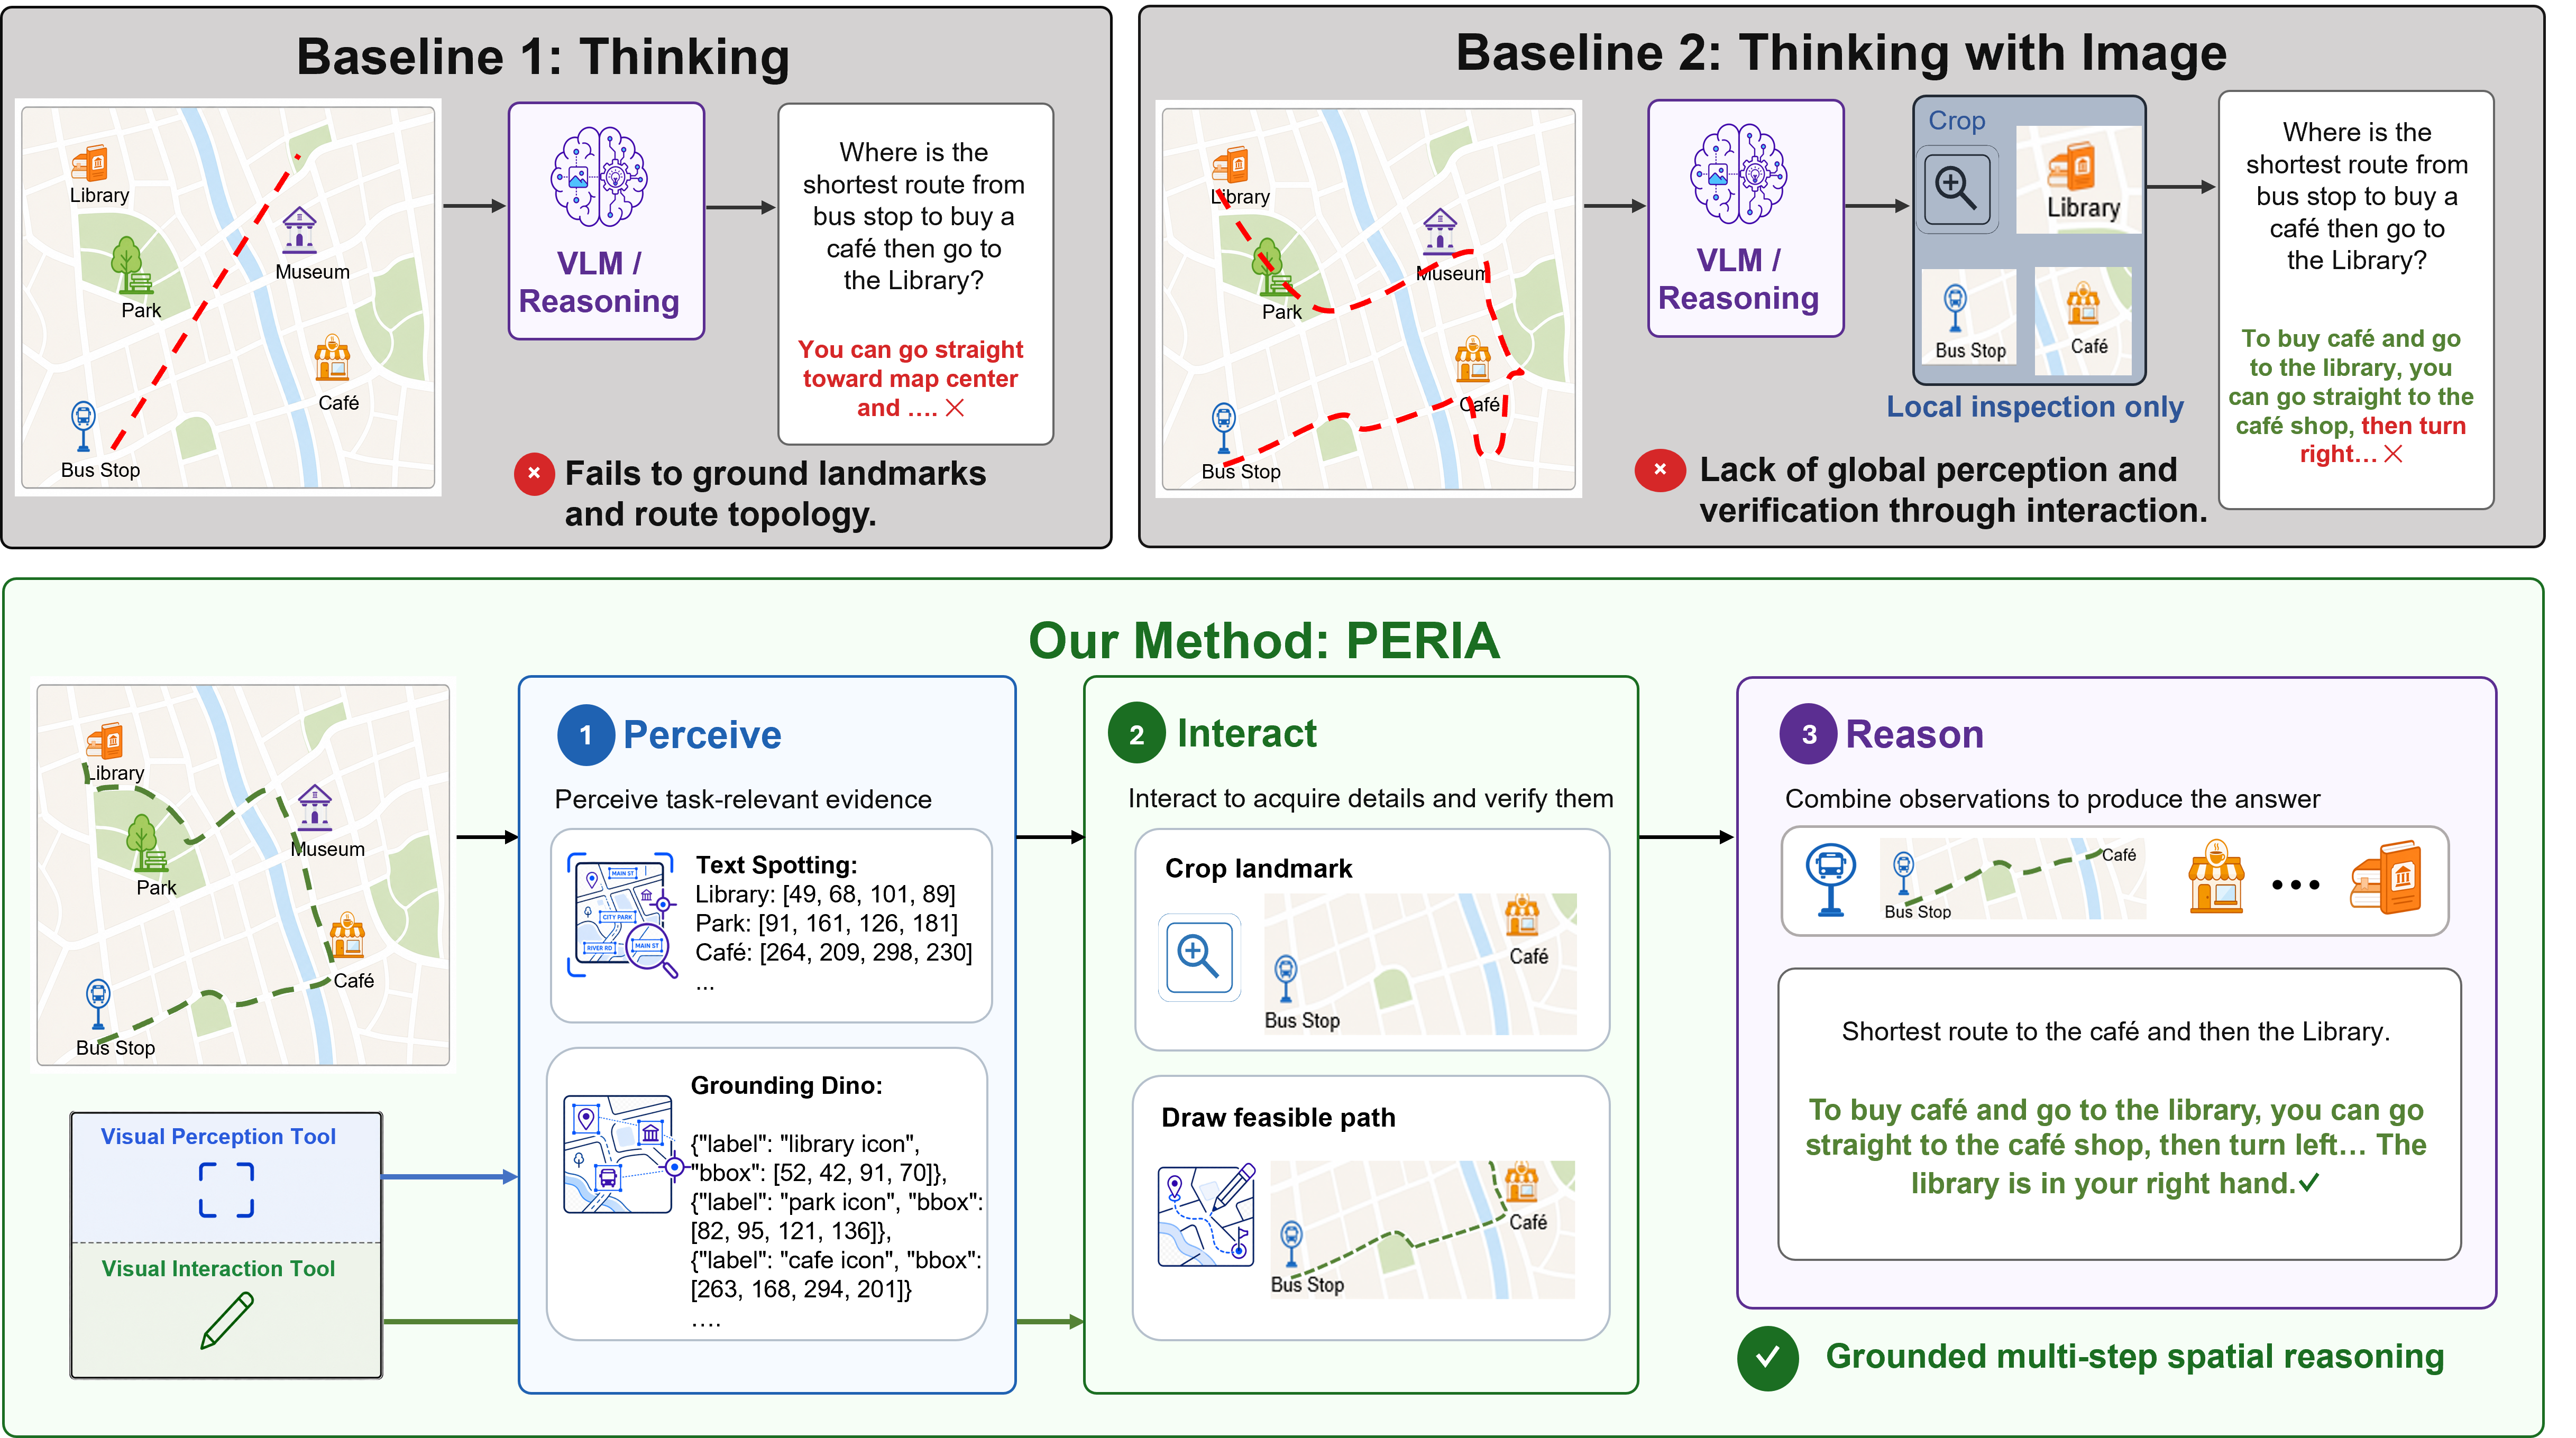
\includegraphics[width=\linewidth]{assets/figure1.png}
\end{center}
\end{columns}

\vspace{1em}
\centering
\colorbox{neuripsred!20}{\parbox{0.9\textwidth}{\centering
\textbf{Key Insight:} Active evidence acquisition through tools is essential for spatial reasoning
}}
\end{frame}

% Slide 2: Our Solution - PERIA
\begin{frame}{PERIA: PERception-Interaction-reason Agent}
\begin{center}
\textbf{A tool-augmented visual agent with two key components:}
\end{center}

\vspace{0.5em}

\begin{columns}[c]
\column{0.48\textwidth}
\centering
\colorbox{blue!10}{\parbox{0.9\textwidth}{
\centering
\textbf{Vision Perception Tools}\\[0.5em]
Extract evidence from images:
\begin{itemize}
    \item Text spotting \& OCR
    \item Map-optimized reading
    \item Object segmentation
    \item Presence verification
\end{itemize}
}}

\column{0.48\textwidth}
\centering
\colorbox{green!10}{\parbox{0.9\textwidth}{
\centering
\textbf{Vision Interaction Tools}\\[0.5em]
Manipulate visual context:
\begin{itemize}
    \item Path drawing
    \item Bounding box annotation
    \item Image cropping
    \item Region focusing
\end{itemize}
}}
\end{columns}

\vspace{1em}
\begin{center}
\colorbox{neuripsblue!20}{\parbox{0.85\textwidth}{\centering
\textbf{18 tools + 3 lightweight tool agents} organized into a modular sandbox
}}
\end{center}
\end{frame}

% Slide 3: Method Overview
\begin{frame}{Training Pipeline: From Tool Sandbox to OR-GIGPO}
\begin{center}
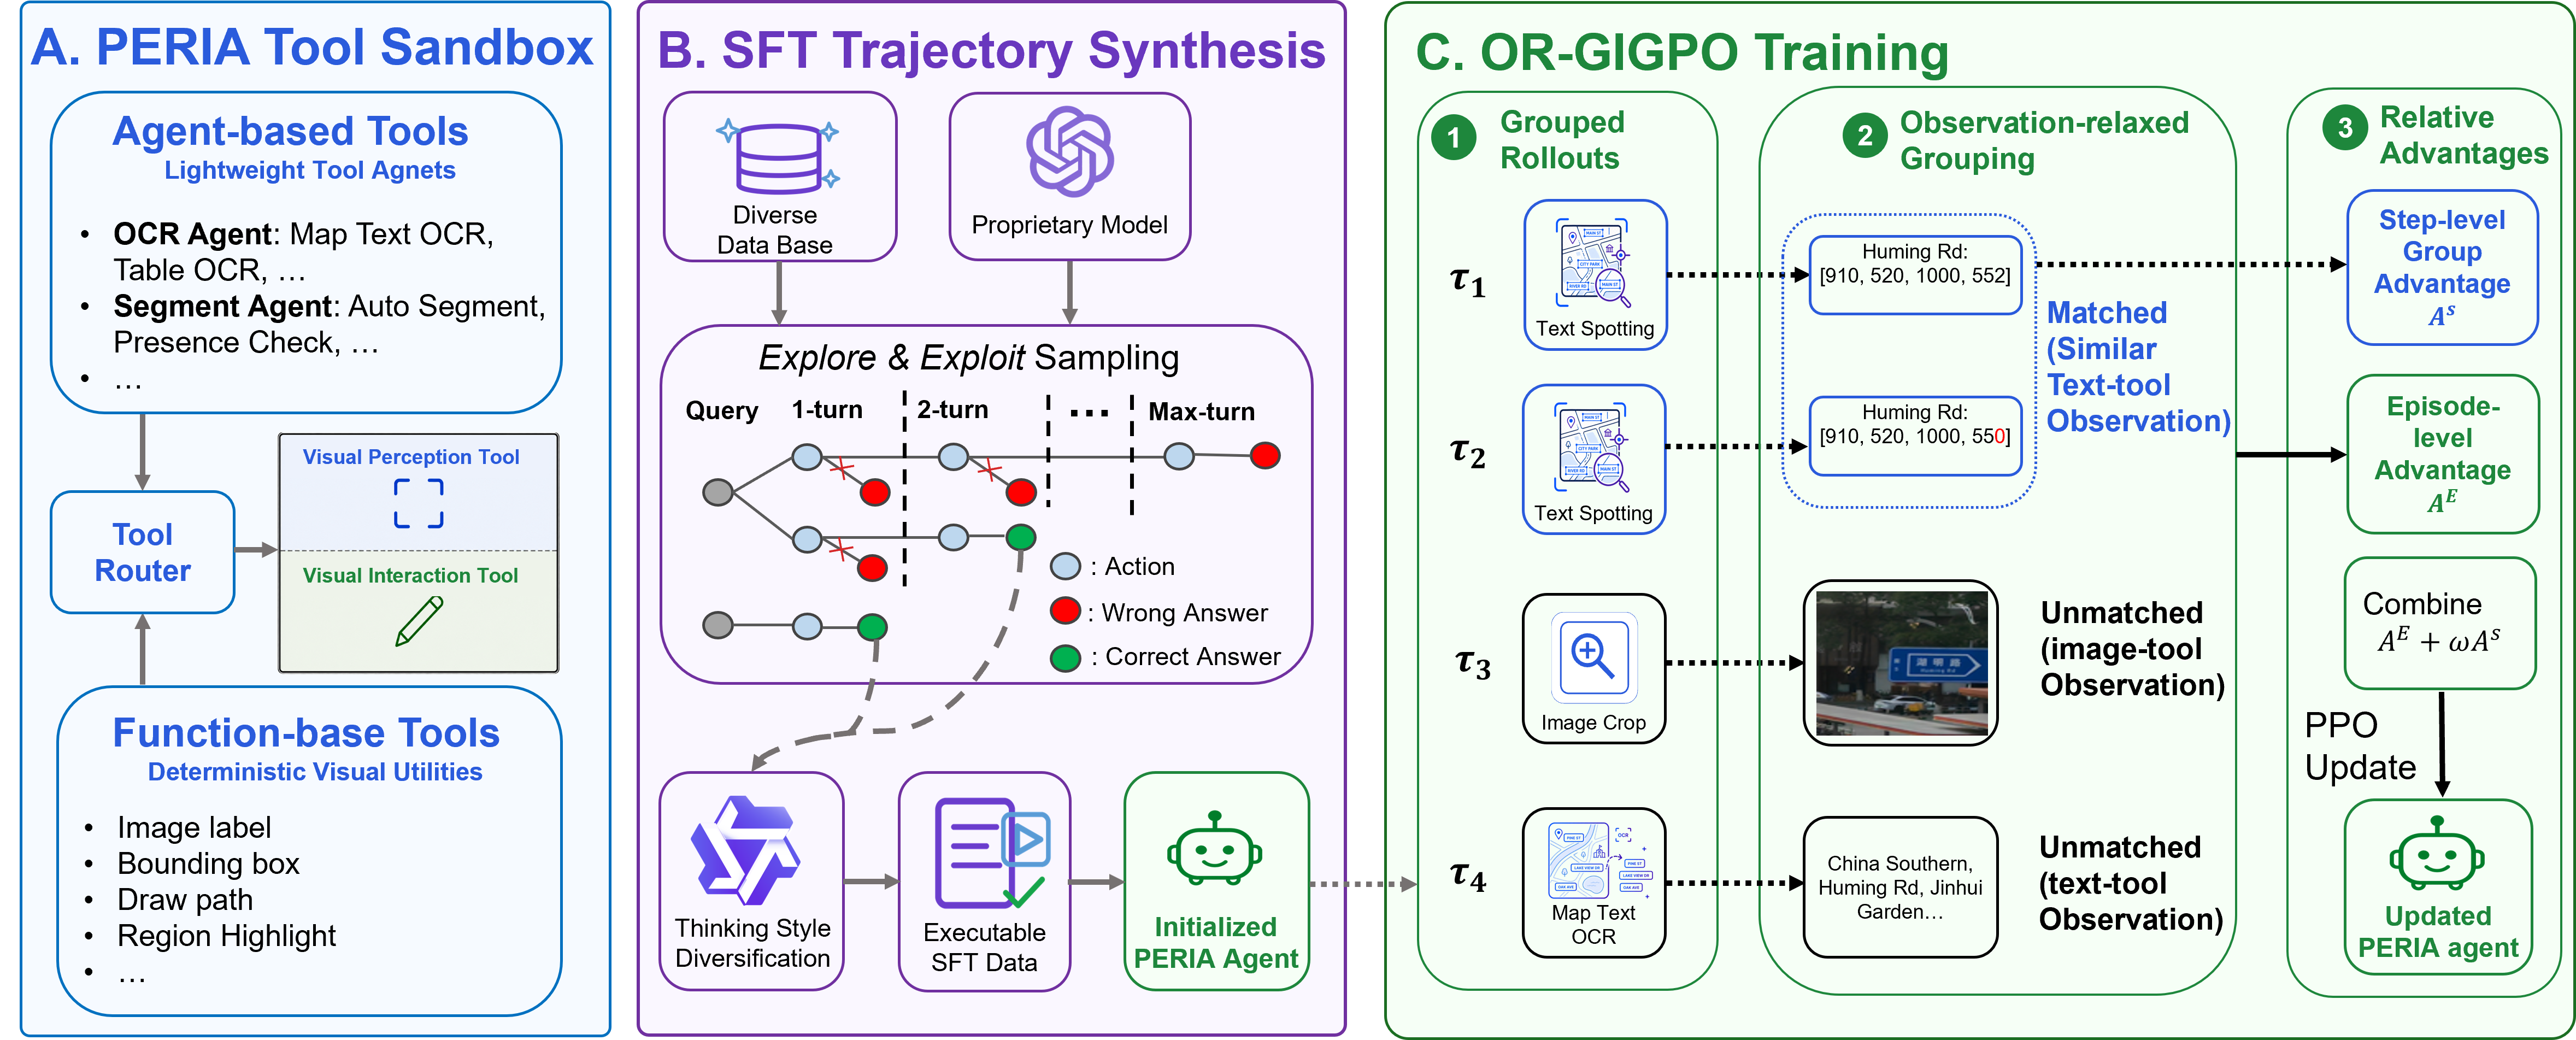
\includegraphics[width=0.9\linewidth]{assets/figure2.png}
\end{center}

\vspace{0.5em}

\begin{enumerate}
    \item \textbf{Tool Sandbox Construction:} Modular perception \& interaction tools
    \item \textbf{SFT Trajectory Synthesis:} Explore-exploit with GPT-5 + thinking diversification
    \item \textbf{OR-GIGPO Training:} Group-in-group optimization with relaxed observations
\end{enumerate}
\end{frame}

% Slide 4: OR-GIGPO Algorithm
\begin{frame}{OR-GIGPO: Observation-Relaxed Group-in-Group Policy Optimization}
\textbf{Challenge:} Multi-step tool-use trajectories need fine-grained credit assignment

\vspace{0.5em}

\textbf{Solution: OR-GIGPO}
\begin{itemize}
    \item \textbf{Group-in-Group:} Sample $N$ rollouts per state, group by relaxed observations
    \item \textbf{Relaxed Observations:} Remove tool outputs, keep only actions \& thoughts
    \item \textbf{Composite Advantages:} Combine step-level and episode-level signals
\end{itemize}

\vspace{0.5em}

\begin{equation*}
A_t^{\text{OR-GIGPO}} = \underbrace{\frac{1}{G}\sum_{i=1}^G \left(r_t^{(i)} + \gamma V(s_{t+1}^{(i)}) - V(s_t)\right)}_{\text{Step-level advantage}} + \underbrace{\frac{1}{N}\sum_{j=1}^N \left(R^{(j)} - b\right)}_{\text{Episode-level advantage}}
\end{equation*}

\vspace{0.5em}

\centering
\colorbox{neuripsblue!20}{\parbox{0.85\textwidth}{\centering
\textbf{Enables effective multi-tool composition without full observation matching}
}}
\end{frame}

% Slide 5: Results - Main Table
\begin{frame}{Results: Strong Performance Across 13 Benchmarks}
\begin{center}
\textbf{PERIA-8B vs. State-of-the-Art Models}
\end{center}

\vspace{-0.5em}

\begin{table}[h]
\centering
\small
\begin{tabular}{lcccc}
\toprule
\textbf{Model} & \textbf{Size} & \textbf{In-Dist.} & \textbf{Out-of-Dist.} & \textbf{Avg.} \\
\midrule
Qwen3-VL-Thinking & 8B & 44.1 & 31.7 & 37.4 \\
InternVL3.5 & 8B & 39.2 & 28.5 & 33.4 \\
VTool-R1 & 7B & 41.8 & 29.3 & 35.0 \\
Mini-o3 & 7B & 42.5 & 30.8 & 36.2 \\
\midrule
\textbf{PERIA-8B (Ours)} & \textbf{8B} & \textbf{54.1} & \textbf{36.1} & \textbf{44.4} \\
\textcolor{neuripsred}{\textit{$\Delta$ vs. Backbone}} & & \textcolor{neuripsred}{\textit{+10.0}} & \textcolor{neuripsred}{\textit{+4.4}} & \textcolor{neuripsred}{\textit{+7.0}} \\
\midrule
Qwen3-VL-Thinking & 235B-A22B & 56.3 & 37.2 & 46.0 \\
GPT-5 & - & 58.1 & 38.5 & 47.5 \\
\bottomrule
\end{tabular}
\end{table}

\vspace{0.5em}

\begin{columns}[c]
\column{0.5\textwidth}
\begin{itemize}
    \item \textcolor{neuripsred}{\textbf{+10.0\%}} on in-distribution tasks
    \item \textcolor{neuripsred}{\textbf{+4.4\%}} on out-of-distribution tasks
\end{itemize}

\column{0.5\textwidth}
\begin{itemize}
    \item \textbf{7.0\%--14.8\%} better than SOTA at similar size
    \item Approaches 235B models performance
\end{itemize}
\end{columns}
\end{frame}

% Slide 6: Results - Per Dataset
\begin{frame}{Performance Across Task Families}
\begin{center}
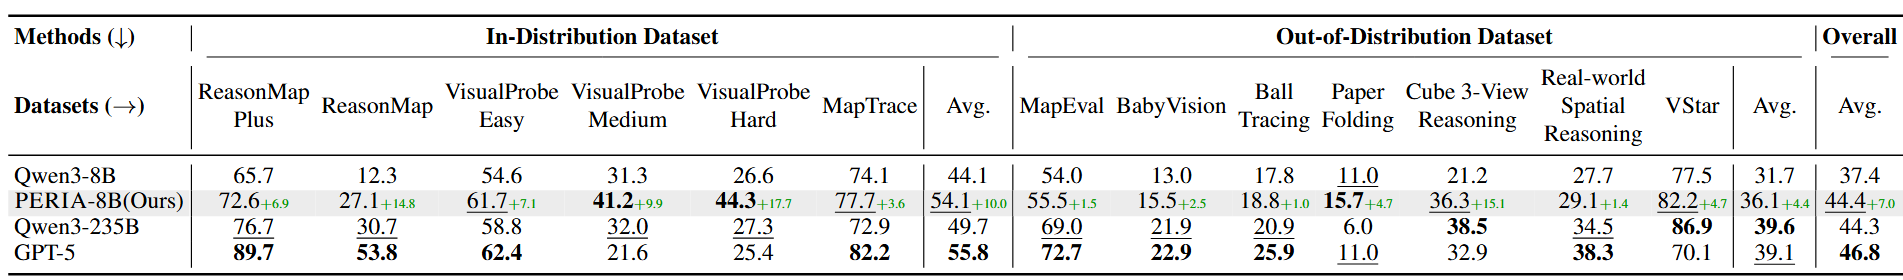
\includegraphics[width=0.95\linewidth]{assets/image.png}
\end{center}

\vspace{-0.5em}

\textbf{Strong results across diverse spatial reasoning tasks:}
\begin{itemize}
    \item \textbf{Map Reasoning:} ReasonMap, ReasonMap-Plus, MapTrace, MapEval
    \item \textbf{Visual Probing:} Multi-object tracking and localization
    \item \textbf{3D Reasoning:} Cube views, paper folding, real-world spatial
    \item \textbf{Vision Reconstruction:} Ball tracking, BabyVision, V*
\end{itemize}
\end{frame}

% Slide 7: Ablation Studies
\begin{frame}{Ablation Studies: What Matters?}
\begin{columns}[c]
\column{0.48\textwidth}
\textbf{Training Recipe:}
\begin{itemize}
    \item \textbf{w/o RL:} 40.4\% $\rightarrow$ \textbf{Full:} 44.4\%
    \begin{itemize}
        \item RL adds \textcolor{neuripsred}{+4.0\%} overall
        \item Especially strong on ID tasks (+7.2\%)
    \end{itemize}
    \item \textbf{w/o SFT:} 40.7\% (RL from scratch)
    \begin{itemize}
        \item SFT establishes tool competence
        \item RL refines multi-step reasoning
    \end{itemize}
\end{itemize}

\column{0.48\textwidth}
\textbf{OR-GIGPO Components:}
\begin{itemize}
    \item \textbf{vs. PPO:} +2.8\% improvement
    \item \textbf{vs. GRPO:} +1.5\% improvement
    \item \textbf{Relaxed Obs:} Critical for grouping
    \item \textbf{Composite Adv:} Balances short/long term
\end{itemize}

\vspace{1em}
\centering
\colorbox{neuripsblue!20}{\parbox{0.9\textwidth}{\centering
Both SFT \& RL stages\\are essential
}}
\end{columns}
\end{frame}

% Slide 8: Qualitative Examples
\begin{frame}{Qualitative Example: Multi-Step Tool Use}
\begin{center}
\textbf{Task:} Plan a subway route from Station A to Station D
\end{center}

\vspace{0.5em}

\begin{enumerate}
    \item \textbf{Perception:} Use \texttt{map\_text\_ocr} to extract all station names
    \begin{itemize}
        \item Result: Identified 15 stations and 3 transfer points
    \end{itemize}

    \item \textbf{Interaction:} Use \texttt{draw\_path} to trace potential routes
    \begin{itemize}
        \item Result: Generated 2 candidate paths
    \end{itemize}

    \item \textbf{Reasoning:} Compare route lengths and transfer counts
    \begin{itemize}
        \item Result: Route via Station B (1 transfer, shorter)
    \end{itemize}

    \item \textbf{Verification:} Use \texttt{bounding\_box} to verify connections
    \begin{itemize}
        \item Result: Confirmed all connections are valid
    \end{itemize}
\end{enumerate}

\vspace{0.5em}
\centering
\colorbox{green!20}{\parbox{0.85\textwidth}{\centering
\textbf{PERIA correctly solves the task through active tool composition}
}}
\end{frame}

% Slide 9: Key Contributions
\begin{frame}{Key Contributions}
\begin{enumerate}
    \item \textbf{PERIA Framework:} A modular tool-augmented visual agent for spatial reasoning
    \begin{itemize}
        \item 18 perception \& interaction tools
        \item Unified POMDP formulation
    \end{itemize}

    \vspace{0.5em}

    \item \textbf{OR-GIGPO Algorithm:} Novel RL method for multi-tool composition
    \begin{itemize}
        \item Observation-relaxed grouping
        \item Composite advantage estimation
    \end{itemize}

    \vspace{0.5em}

    \item \textbf{Strong Empirical Results:} State-of-the-art on 13 benchmarks
    \begin{itemize}
        \item +10.0\% over backbone on in-distribution tasks
        \item Approaches 30$\times$ larger models
    \end{itemize}

    \vspace{0.5em}

    \item \textbf{Open Resources:} Code, models, and datasets released
    \begin{itemize}
        \item Reproducible training pipeline
        \item Extensible tool sandbox
    \end{itemize}
\end{enumerate}
\end{frame}

% Slide 10: Limitations and Future Work
\begin{frame}{Limitations and Future Directions}
\textbf{Current Limitations:}
\begin{itemize}
    \item Tool sandbox currently focused on 2D spatial reasoning
    \item Limited to 18 tools (though easily extensible)
    \item OR-GIGPO requires significant compute for RL training
\end{itemize}

\vspace{1em}

\textbf{Future Directions:}
\begin{itemize}
    \item \textbf{Broader Tool Coverage:} 3D manipulation, video understanding
    \item \textbf{More Efficient Training:} Distillation, data efficiency improvements
    \item \textbf{Compositional Generalization:} Zero-shot tool composition
    \item \textbf{Multi-Modal Extensions:} Audio, text, embodied environments
\end{itemize}

\vspace{1em}
\centering
\colorbox{neuripsblue!20}{\parbox{0.85\textwidth}{\centering
\textbf{Vision:} General-purpose tool-augmented visual agents for any reasoning task
}}
\end{frame}

% Slide 11: Conclusion
\begin{frame}{Conclusion}
\begin{center}
\Large
\textbf{PERIA: Tool-Augmented Visual Agents for Spatial Reasoning}
\end{center}

\vspace{1em}

\begin{columns}[c]
\column{0.5\textwidth}
\textbf{What we built:}
\begin{itemize}
    \item Modular tool sandbox
    \item SFT trajectory synthesis
    \item OR-GIGPO training algorithm
    \item 8B model $\approx$ 235B baseline
\end{itemize}

\column{0.5\textwidth}
\textbf{What we learned:}
\begin{itemize}
    \item Tools enable evidence acquisition
    \item SFT + RL both essential
    \item Relaxed grouping helps credit
    \item Strong generalization
\end{itemize}
\end{columns}

\vspace{2em}

\begin{center}
\Large
\textbf{Thank You!}\\[1em]
\normalsize
\textbf{Paper:} \url{https://arxiv.org/abs/2606.12830}\\
\textbf{Code:} \url{https://github.com/antoinegg1/PEDIA}\\
\textbf{Project Page:} \url{https://antoinegg1.github.io/PEDIA/}
\end{center}
\end{frame}

\end{document}
